
% controlled-assessments.tex - Our first LaTeX example!

%%%%%%%%%%%%%%%%%%%%%%%%%%%%%%%%%%%%%%%%%
% Beamer Presentation
% LaTeX Template
% Version 1.0 (10/11/12)
%
% This template has been downloaded from:
% http://www.LaTeXTemplates.com
%
% License:
% CC BY-NC-SA 3.0 (http://creativecommons.org/licenses/by-nc-sa/3.0/)
%
%%%%%%%%%%%%%%%%%%%%%%%%%%%%%%%%%%%%%%%%%

%----------------------------------------------------------------------------------------
%	PACKAGES AND THEMES
%----------------------------------------------------------------------------------------

\documentclass{beamer}
\mode<presentation> {

% The Beamer class comes with a number of default slide themes
% which change the colors and layouts of slides. Below this is a list
% of all the themes, uncomment each in turn to see what they look like.

%\usetheme{default}
%\usetheme{AnnArbor}
%\usetheme{Antibes}
%\usetheme{Bergen}
%\usetheme{Berkeley}
%\usetheme{Berlin}
%\usetheme{Boadilla}
%\usetheme{CambridgeUS}
%\usetheme{Copenhagen}
%\usetheme{Darmstadt}
%\usetheme{Dresden}
%\usetheme{Frankfurt}
%\usetheme{Goettingen}
%\usetheme{Hannover}
%\usetheme{Ilmenau}
%\usetheme{JuanLesPins}
%\usetheme{Luebeck}
\usetheme{Madrid}
%\usetheme{Malmoe}
%\usetheme{Marburg}
%\usetheme{Montpellier}
%\usetheme{PaloAlto}
%\usetheme{Pittsburgh}
%\usetheme{Rochester}
%\usetheme{Singapore}
%\usetheme{Szeged}
%\usetheme{Warsaw}

% As well as themes, the Beamer class has a number of color themes
% for any slide theme. Uncomment each of these in turn to see how it
% changes the colors of your current slide theme.
\definecolor{mypurplish}{rgb}{0.3, 0.12, 0.4}
%\usecolortheme{albatross}
%\usecolortheme{beaver}
%\usecolortheme{beetle}
%\usecolortheme{crane}
%\usecolortheme{dolphin}
%\usecolortheme{dove}
%\usecolortheme{fly}
%\usecolortheme{lily}
%\usecolortheme{orchid}
%\usecolortheme{rose}
%\usecolortheme{seagull}
%\usecolortheme{seahorse}
%\usecolortheme{spruce}
%\usecolortheme{whale}
%\usecolortheme{wolverine}
\usecolortheme[named=mypurplish]{structure}
%\setbeamertemplate{footline} % To remove the footer line in all slides uncomment this line
%\setbeamertemplate{footline}[page number] % To replace the footer line in all slides with a simple slide count uncomment this line

%\setbeamertemplate{navigation symbols}{} % To remove the navigation symbols from the bottom of all slides uncomment this line
}
\usepackage{graphicx} % Allows including images
\usepackage{booktabs} % Allows the use of \toprule, \midrule and \bottomrule in tables
\usepackage{tikz}



\newcommand\RBox[1]{%
  \tikz\node[draw,rounded corners,align=center,] {#1};%
}  
\usepackage{color}
\usepackage{listings}
\usepackage{setspace}

\usepackage[framemethod=tikz]{mdframed}



\definecolor{Code}{rgb}{0,0,0}
\definecolor{Decorators}{rgb}{0.2,0.2,0.2}
\definecolor{Numbers}{rgb}{0.5,0,0}
\definecolor{MatchingBrackets}{rgb}{0.25,0.5,0.5}
\definecolor{Keywords}{rgb}{0,0,1}
\definecolor{self}{rgb}{1,0,0}
\definecolor{Strings}{rgb}{0,0.63,0}
\definecolor{Comments}{rgb}{0,0.63,1}
\definecolor{Backquotes}{rgb}{0,0.2,0}
\definecolor{Classname}{rgb}{0,0,1}
\definecolor{FunctionName}{rgb}{1,0,1}
\definecolor{Operators}{rgb}{0,0,0}
\definecolor{Background}{rgb}{0.95,0.95,0.95}


            
\lstset{
numbers=left,
numberstyle=\footnotesize,
numbersep=1em,
xleftmargin=1em,
framextopmargin=2em,
framexbottommargin=2em,
showspaces=false,
showtabs=false,
showstringspaces=false,
frame=l,
tabsize=4,
breaklines=true,
postbreak=\raisebox{0ex}[0ex][0ex]{\ensuremath{\color{red}\hookrightarrow\space}},
% Basic
basicstyle=\ttfamily\small\setstretch{1},
backgroundcolor=\color{Background},
language=Python,
% Comments
commentstyle=\color{Comments},
% Strings
stringstyle=\color{Strings},
morecomment=[s][\color{Strings}]{"""}{"""},
morecomment=[s][\color{Strings}]{'''}{'''},
% keywords
morekeywords={import,from,class,def,for,while,if,is,in,elif,else,not,and,or,print,break,continue,return,True,False,None,access,as,,del,except,exec,finally,global,import,lambda,pass,print,raise,try,assert},
keywordstyle={\color{Keywords}\bfseries},
% additional keywords
morekeywords={[2]@invariant},
keywordstyle={[2]\color{Decorators}\slshape},
emph={self},
emphstyle={\color{self}\slshape},
%
}{}

\title[Python in Ed]{Python in Education}
\author[Dave Ames]{Dave Ames}
\institute[CAS]{Computing At School}


\begin{document}

{
  \usebackgroundtemplate{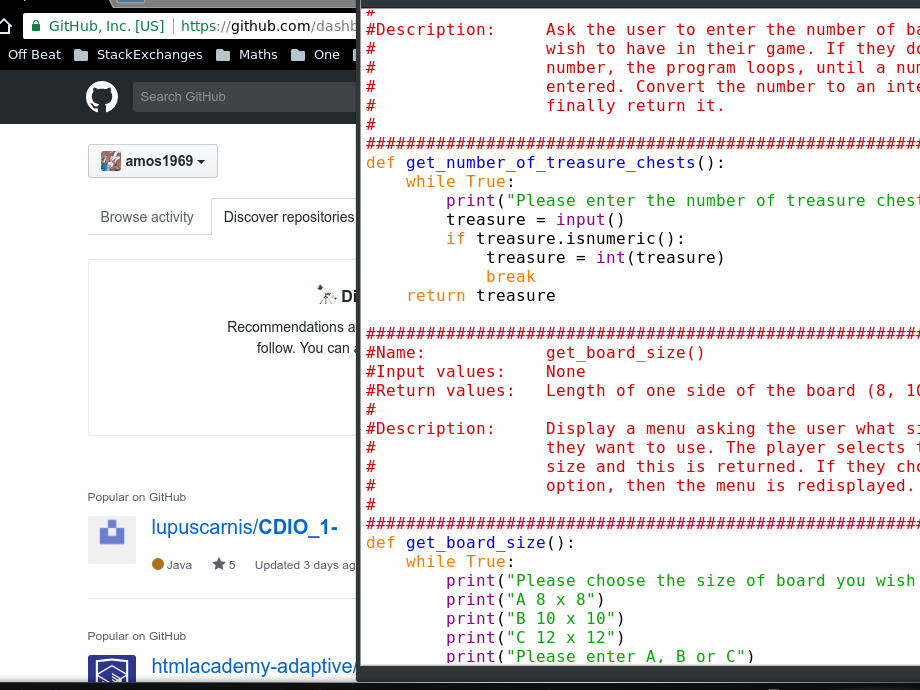
\includegraphics[width=1.0\paperwidth]{front_slide.png}}
  \begin{frame}[plain]
    \vspace{2cm}
    \centering
\begin{mdframed}[tikzsetting={draw=mypurplish,fill=white,fill opacity=0.8,
               line width=3pt},backgroundcolor=none,leftmargin=20,
               rightmargin=20,innertopmargin=8pt,roundcorner=15pt]
               {\huge \inserttitle} \\
               \insertauthor  \hspace{0.4cm}  (\insertinstitute) \hspace{0.3cm}  \insertdate \\
               \href{mailto:dave.ames@computingatschool.org.uk}{E: dave.ames@computingatschool.org.uk} \hspace{0.2cm}
               \href{http://twitter.com/davidames}{T: @DavidAmes}
               
             \end{mdframed}
\end{frame}
}


\section{Main part}

\begin{frame}
\frametitle{My Role(s)}
\subsection{My Role(s)}
\begin{itemize}
\item Regional Coordinator and Master Teacher for the CAS Regional Centre at University of Manchester
  \pause
\item Regional Coordinator and Master Teacher for the CAS Regional Centre at Lancaster University
  \pause
\item Liaison Tutor for Maths and Computing Trainee Teachers at Knutsford Academy (attached to LJMU)
  \pause
\item Associate Tutor for Computing Trainees on the PGCE in Computer Science/ICT at MMU
  \pause
\item Consultant for the National STEM Centre in York (deliver CPD and create resources)
  \pause
\item eTutor for the BCS Certificate in Teaching Computer Science
  \pause 
\end{itemize}
\end{frame}


\begin{frame}
\frametitle{My background}
\subsection{My background}

\begin{itemize}
  \pause
\item Programmed in the 80s on 48k ZX Spectrum at home and TRS80s at school both in Basic
  \pause
\item Maths Teacher
  \pause
\item Part Time Degree in Computing at Bolton - mainly C++ some VB6
  \pause
\item Played with PyQt and Pygame around the end of my degree (early 2009)
  \pause
\item Created and administered our School website in Django (2009-2013ish)
\end{itemize}

\end{frame}


\begin{frame}
  \frametitle{The Change to Computing - 2012}
  \subsection{The Change to Computing - 2012}

  \begin{itemize}
    \pause
  \item NextGen Report by Ian Livingstone \url{http://www.nesta.org.uk/publications/next-gen}
    \pause
  \item Shut Down or Restart? Report by Steve Furber and others
    \url{https://royalsociety.org/topics-policy/projects/computing-in-schools/report/}
    \pause
  \item Speech by Senior Google Official condemning ICT as ``not fit for purpose''
    \pause
  \item September 2012 - disapplication of ICT as a subject, with new ``Computing'' subject coming on stream in
    September 2014    
  \end{itemize}
\end{frame}

\begin{frame}
  \frametitle{A New Era of Computing in Schools?}
  \subsection{A New Era of Computing in Schools?}
  \begin{itemize}
    \pause
  \item Computing at School - up to 2012 (2000ish members, 20-30 Hubs)
    \pause
  \item Launched the Network of Excellence in Teaching Computer Science in 2012 - Added Master Teachers to the mix
    \pause
  \item Now have 28341 members, and 248 Hubs. Plus somewhere in the region of 450 Master Teachers. With 10 Regional
    Centres in England (and CAS in the devolved nations)
    \pause
  \item National Curriculum for Computing at Key Stage 3 specifies that students should learn two programming languages
    at least one of which is text based
    \pause
  \item Anecdotally approximately 75-80\% of the schools I deal with are using Python as their main text based language
    \pause
  \item Key Stage 4 (GCSE) - each of the major exam boards has a GCSE, (new versions are being examined for the first
    time this summer)
  \end{itemize}
 
\end{frame}

\begin{frame}
\frametitle{GCSE and Beyond}
\subsection{GCSE and Beyond}
\begin{itemize}
  \item At GCSE all of the boards now have a practical programming component worth 20\% of the final grade known as NEA
    Tasks (previously called Controlled Assessments)
    \pause
  \item These have issues!
    \pause
  \item I have some to show you after.
    \pause
  \item A Level also has a 20\% NEA, but these are personal projects and work much better
    \pause
  \item However the skills required to access the highest grades are quite high
    \pause
  \item Still no blanket requirement to have studied A Level Computer Science to do a degree in it, is hampering
    adoption.   
\end{itemize}

\end{frame}


\begin{frame}
\frametitle{What can you do?}
\subsection{What can you do?}
\begin{itemize}
\item Volunteer with organisations like CodeClub and CoderDojo to work with children
  \pause
\item Become a STEM Ambassador
  \pause
\item Encourage your company to do outreach to schools and similar organisations
  \pause
\item Volunteer with adult coding organisations such as DjangoGirls and Code Up
  \pause
\item Currently trialling sessions with Hive Manchester and developers from Autotrader/Rental Cars for
  teachers. Potential to utilise some of you to deliver similar sessions
  \pause
\item If you're interested email me at \url{dave.ames@computingatschool.org.uk}
\end{itemize}

\end{frame}

  
\begin{frame}
\begin{center}
\begin{huge}
  \texttt{Questions?}
\end{huge}
\end{center}
\normalfont
\end{frame}

\begin{frame}
\begin{center}
  \begin{huge}
    \url{https://goo.gl/1mnpKo}
\end{huge}
\end{center}
\normalfont
\end{frame}

\end{document}

%%% Local Variables:
%%% mode: latex
%%% TeX-master: t
%%% End:
